\section{Evaluation}
\label{sec:evaluation}
\label{Simulation Result}
\indent 
	We conduct a simulation using the procedure described above. We put four robots in the simulation field and draw three range, representing the sensory range, communication range, and rejection range, for each robots. We draw straight lines between robots with the average signal strength of four antenna of robots between them instead of the signal strength of each robots for a better visualization. In this simulation we assumed following:
\begin{itemize}
	\item The frequency of the transceiver is at 2.4 Gigahertz range.
	\item Each robots is using different frequency channel so that each signal cannot interfere another.
	\item The reference distance of the transceiver is 1.8 meters and the receiving power at the reference distance is -27.25 decibel. The standard deviation of the Gaussian white noise is 1, since we do not know the real antenna's Signal-to-Noise Ratio.
	\item The sensory range, the communication range, and the rejection range are 200 meters, 100 meters, and 100 meters respectively.
\end{itemize}
\par
	The example results of the simulation are the following figures: figure 9 and figure 10. Figure 10 shows the signal strength against distance to visualize the relationship between signal strength and distance. Asides from the effect of the White Gaussian Noise and the Fading, it shows that it has a logarithmic relationship. Figure 9 shows four simulation results that the four robots are randomly placed and the average signal strength are measured accordingly. The simulation result in figure 9 shows that the measured average signal strength are measured differently with distance. It also shows that the robots around the communication range has signal strength around -60db, and the robots within the sensory range have signal strength of more than -70db, whereas the signal strength between two robots outside of the sensory range is measured less than -70db. \\
 
\begin{figure}[ht]
	\centering
	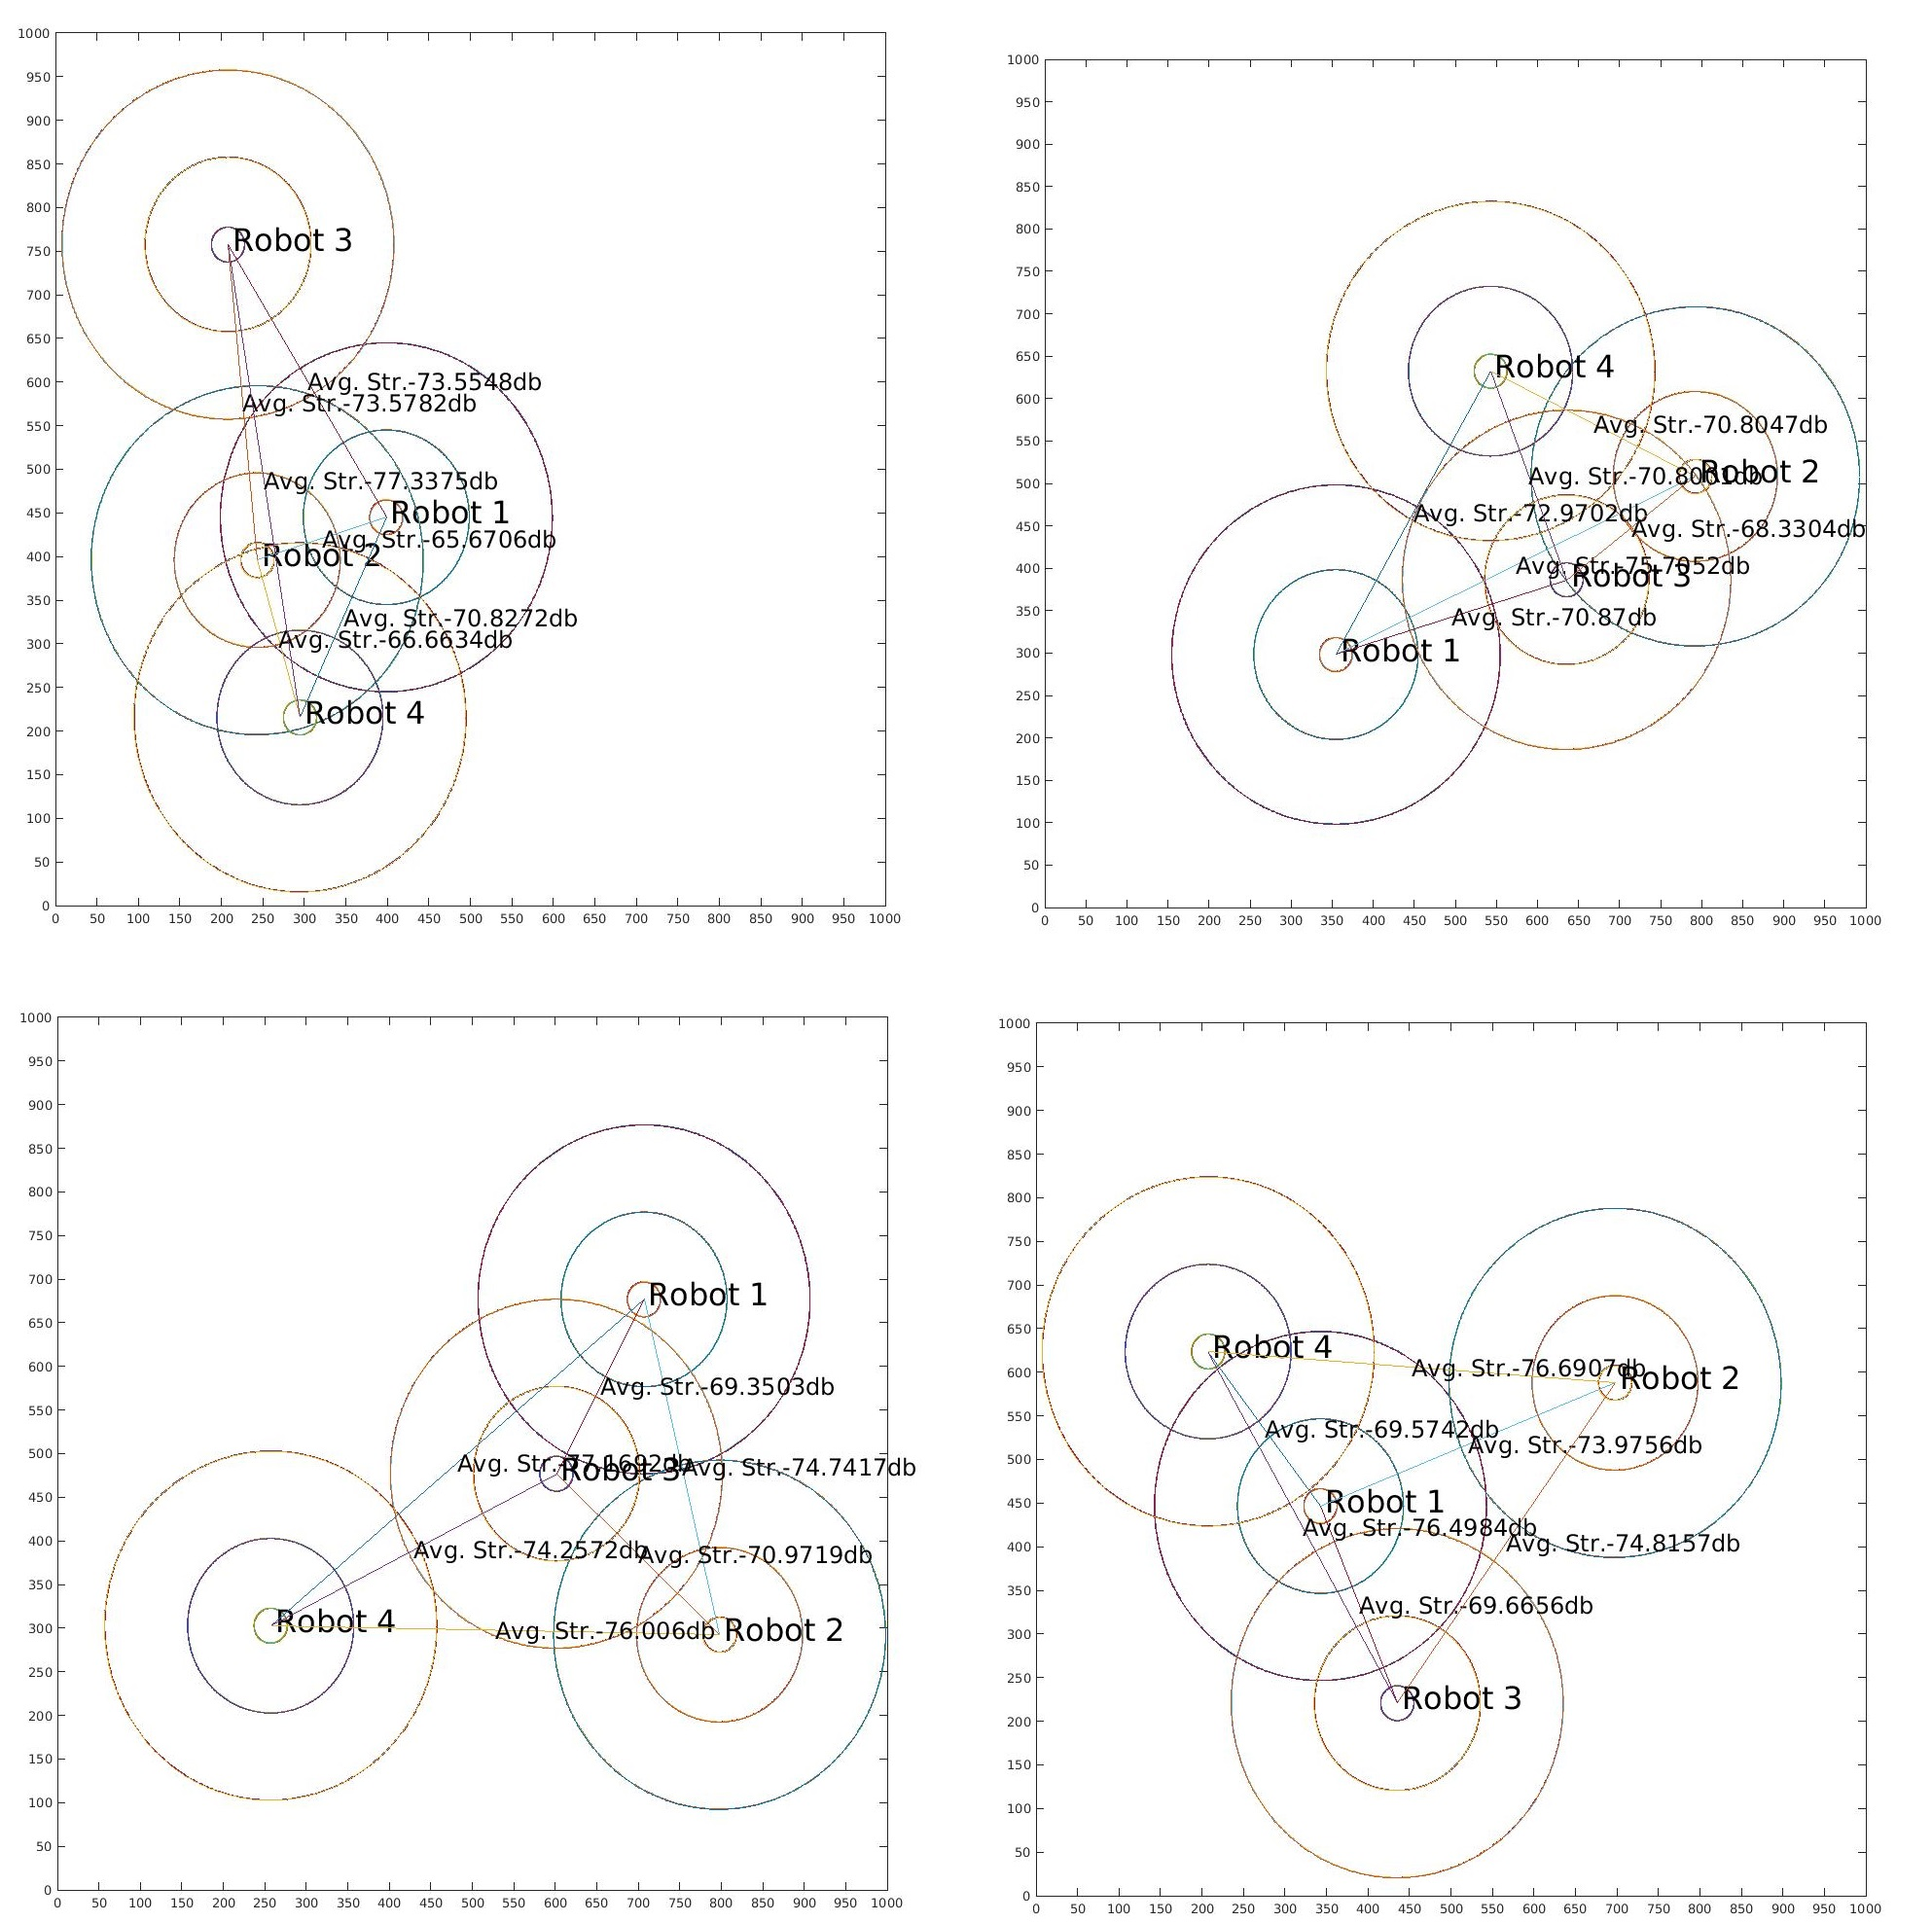
\includegraphics[width=0.4\textwidth]{simulation0}
	\caption{Four sample simulations}
	%\label{fig1}
	\end{figure}
	
\begin{figure}[ht]
	\centering
	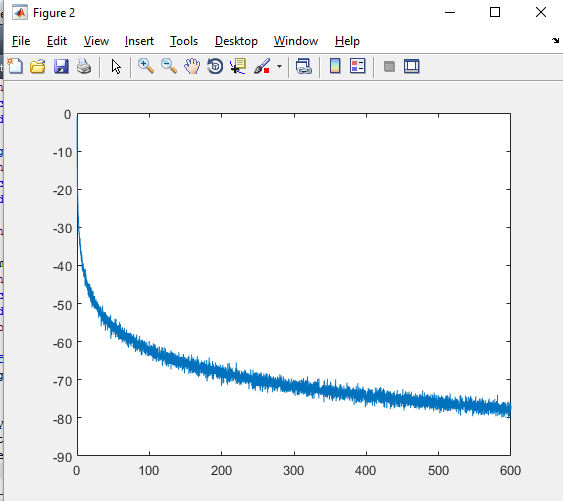
\includegraphics[width=0.4\textwidth]{simulation5}
	\caption{Power vs. Distance}
	%\label{fig1}
	\end{figure}
	


